%% !TEX TS-program = pdflatex
%% !TEX encoding = UTF-8 Unicode
%
%% This is a simple template for a LaTeX document using the "article" class.
%% See "book", "report", "letter" for other types of document.
%%\documentclass{acm_proc_article-sp} % use larger type; default would be 10pt
%\documentclass{article}
%\usepackage[utf8]{inputenc} % set input encoding (not needed with XeLaTeX)
%\usepackage{setspace}
%%\doublespacing
%%%% Examples of Article customizations
%% These packages are optional, depending whether you want the features they provide.
%% See the LaTeX Companion or other references for full information.
%
%%%% PAGE DIMENSIONS
%%\usepackage{geometry} % to change the page dimensions
%%\geometry{a4paper} % or letterpaper (US) or a5paper or....
%% \geometry{margin=2in} % for example, change the margins to 2 inches all round
%% \geometry{landscape} % set up the page for landscape
%%   read geometry.pdf for detailed page layout information
%\usepackage{multirow}
%\usepackage{graphicx} % support the \includegraphics command and options
%
%% \usepackage[parfill]{parskip} % Activate to begin paragraphs with an empty line rather than an indent
%
%%%% PACKAGES
%\usepackage{booktabs} % for much better looking tables
%\usepackage{array} % for better arrays (eg matrices) in maths
%\usepackage{paralist} % very flexible & customisable lists (eg. enumerate/itemize, etc.)
%\usepackage{verbatim} % adds environment for commenting out blocks of text & for better verbatim
%\usepackage{subfig} % make it possible to include more than one captioned figure/table in a single float
%% These packages are all incorporated in the memoir class to one degree or another...
%
%%%% HEADERS & FOOTERS
%\usepackage{fancyhdr} % This should be set AFTER setting up the page geometry
%\pagestyle{fancy} % options: empty , plain , fancy
%\renewcommand{\headrulewidth}{0pt} % customise the layout...
%\lhead{}\chead{}\rhead{}
%\lfoot{}\cfoot{\thepage}\rfoot{}
%
%%%% SECTION TITLE APPEARANCE
%%\usepackage{sectsty}
%%\allsectionsfont{\sffamily\mdseries\upshape} % (See the fntguide.pdf for font help)
%% (This matches ConTeXt defaults)
%
%%%% ToC (table of contents) APPEARANCE
%%\usepackage[nottoc,notlof,notlot]{tocbibind} % Put the bibliography in the ToC
%%\usepackage[titles,subfigure]{tocloft} % Alter the style of the Table of Contents
%%\renewcommand{\cftsecfont}{\rmfamily\mdseries\upshape}
%%\renewcommand{\cftsecpagefont}{\rmfamily\mdseries\upshape} % No bold!
%
%%%% END Article customizations
%
%%%% The "real" document content comes below...
%
%\title{Increasing the spread of health information on social media}
%\author{Todd Bodnar and Marcel Salath\'e}%\affil{1}{}\affil{2}{EPFL}}
%%\date{} % Activate to display a given date or no date (if empty),
%         % otherwise the current date is printed 
%
%\begin{document}
%\maketitle

\chapter{Beyond Network and Sentiment Analysis for Retweet Prediction}
\label{retweets}
\section{Introduction}

Up to this point, we have only considered measuring behaviors and disease using social media. However, this knowledge isn't useful if it cannot be used to influence future disease prevalence or behaviors. Here, we consider Twitter as a source of information from which users may gain information about a disease and potentially modify their behaviors that relate to the disease. \cite{salathe2013dynamics,timimi2013shape} For example, previous work has shown that influenza vaccination rates can be inferred from Twitter \cite{salathe2011assessing} and that users modify their sentiment of vaccinations in a way that is statistically related to their exposure to other Tweets about vaccination. \cite{salathe2013dynamics} Thus, a public health official would be interested in exposing as many Twitter users to as many messages about getting vaccinated as a way to \emph{influence} their behavior. \cite{timimi2013shape} A traditional approach to this would be purchasing ad-space, but this can be expensive. Instead, one could post a message on Twitter with the hope that others would read it and find it important enough to share with their friends. However, Twitter users will not blindly retweet a Tweet. Hence, we set out to find factors about a message that would encourage others to further spread the message which a Twitter user could use while crafting her Tweets.

We first collect Tweets from three health related events: the initial announcement of the novel influenza strain H7N9, a measles outbreak that was caused by a subset of the population's refusal to receive the MMR (mumps,measles,rubella) vaccine,\footnote{The vaccine that is incorrectly believed to cause autism.} and Autism Awareness Month. In addition to Tweets, we collected retweets and \emph{inferred} additional message replication through text similarity metrics. These three events were chosen because they all occurred in April 2013---limiting effects of changing Twitter usage--- and because they cover a range of health interests. For example, H7N9 incidence was limited to south east Asia at the time, so the majority of English speaking Twitter users was not directly affected by it. On the other hand, users discussing Autism often were tweeting about someone they know that has the disorder. 

A Twitter user, that is interested in a large impact in one of these public health areas, would want to reach as many people in each of these three target groups. A trivial way to do this would be to send as many messages as possible, however, this is considered bad practice and may annoy others. Instead, several aspects of a message can be crafted to be more appealing to other readers. In this chapter, we consider both aspects that are hard to change (number of followers and what kind of account the message seems to come from) and aspects that are easy to change (message content and sentiment). We find that we are able to accuratly predict how many times a tweet will be retweeted (\(0.4667 \leq r \leq 0.6665\), depending on the dataset).


\section{Background}

The task of predicting a Tweet's propogation is a well studied problem \cite{Suh:2010uw,Ediger:cn,Weng:2012dd,gransee2012,Kim2012retweet,Osborne2011rt,Lerman:2010vo,Anonymous:iQRVCsVz,kwak2010twitter}, even predating Twitter's implementation of retweeting (reposting a message) with the study of, for example, URL's included in a message \cite{kwak2010twitter} or a message's text's simularity to other Tweets \cite{cosme2015,Dou:2012vy}. While the use of alternative methods of finding message propogation has fallen into disuse in the literature since Twitter released an API to detect retweets, we find that the retweet API fails to find about 10\% copies of the message (see table \ref{table:retweetType}). Indeed, Twitter appears to have recently begun removing these near-copies under copyright grounds, as it appears to be a bot strategy.\footnote{http://www.theverge.com/2015/7/25/9039127/twitter-deletes-stolen-joke-dmca-takedown \\ Archived at http://www.webcitation.org/6ajikbuI5} In this chapter, we consider tracking both retweets along with ``hidden'' message reproductions. Preliminary analysis on the H7N9 dataset finds that models perform comparably on both datasets, (see Appendix \ref{appendix:comparetypes}) so here we consider \emph{only} the combined number of times a message is reproduced through either retweets or other methods. 


To determine which attributes are related to higher message reproduction, we first consider four methods others have used to predict retweet count. First, the topology of the follower network is considered \cite{kwak2010twitter,Osborne2011rt}. That is, if a user has more followers, there are more users that may see his messages and may retweet them. This is generally modeled in the form of
\begin{equation}
log(\textrm{retweets}) \propto log(\textrm{out degree})
\end{equation}
due to the long tail distributions of both retweets and out degree \cite{kwak2010twitter}. In this chapter, we only consider models to predict the log-transformed retweet count. Second, we model the influence of different accounts by considering the account's purpose. We label each account as either being a news agency (News), a health organization (Health), a personal account (Personal) or an other account (Other). This was done with a combination of Amazon Mechanical Turk and machine learning. In the H7N9 dataset, we find a strong difference between these different accounts. For example, we find that an average of \(3.98\) Personal accounts retweet each Tweet a health organization posts, but only an average of \(0.0017\) Health accounts retweet each message a Personal account posts. Also of note is that health accounts tend to get more retweets per tweet than news organizations despite having less followers. Third, we consider keyword analysis to predict retweet rates. \cite{gransee2012,Kim2012retweet} For example, Kim et al. \cite{Kim2012retweet} found that tweets that contained vulgarities were less likely to be retweeted. In the H7N9 dataset, we find that more formal phrases such as ``human-to-human'' and ``transmission'' have a positive relation to retweet count while more shocking words like ``killed'' and ``lethal'' actually had a slight negative relation to retweet count, although this could be confounded with the type of account. Fourth, we considered the sentiment expressed in a message as a predictor. \cite{fan2013anger,Kim2012retweet} However, in the H7N9 dataset we were not able to find an effect, possibly due to an overwhelmingly negative sentiment about the topic.

Sentiment analysis has been valuable for many applications such as measuring vaccination rates \cite{salathe2011assessing} or determining political affiliation. \cite{Stieglitz2012politics} However, in the case of infectious disease, sentiment tends to mainly be negative, limiting the power of sentiment analysis. Here, we develop a more general version of sentiment analysis which we base on emotion research and affective science. \cite{Cambria2011,plutchik2001nature} Specifically, we consider Plutchik's model of emotion \cite{plutchik2001nature} which is based on four dimensions: valence, arousal, dominance, and aptitude. Valence corresponds to the attractiveness of a message, which is roughly equivalent to sentiment. Arousal corresponds to the energy behind the message. For example, we may find that messages with multiple exclamation marks show higher arousal than messages with out exclamation marks. Dominance corresponds to how argumentative the message appears.\cite{russell1977evidence} Finally, aptitude corresponds to the inferred maturity of a message.\cite{Thoits:1989va} Note that we are interested in the emotion displayed by the Tweet, which does not necessarily correspond to the emotion of the person that made the tweet. For an example of both extremes of each of these four dimensions see Table 4.

\section{Tweet Collection}
We analyzed 947,967 tweets from March 31, 2013 to April 27, 2013. This period of time included the WHO's announcement of H7N9, autism awareness month, and an outbreak of measles. We did not hit any rate limits, so it is likely that this dataset contains all relevant, public tweets from the timespan. Tweets were selected if they contained one of a set of keywords. We defined the set of H7N9 related tweets as any tweet that contained the word ``H7N9.'' Similarly, we defined the set of autism related tweets as any tweet that contained the word ``autism'', ``autistic'', or ``Aspergers'' and defined the set of measles related tweets as ones that contained the word ``mmr'', ``mumps'', ``measles'', or ``rubella.''  We did not require that the text matched case with the keyword. Each tweet consists of a message of up to 140 characters long, the time it was tweeted, information about the origin tweet, if the tweet is a retweet, and information on the user that posted it, such as the number of her followers and her language. 

\section{Metric Measurement}
\subsection{Retweet Measurement}

Retweets are the reposting of another users' Tweet on one's own Twitter account, generally signaling that the retweeter finds the message interesting enough to pass on to his or her own readers. The definition is somewhat vague, however, as there are multiple ways that a user could choose to repost a message. First, a user can use the build in ``Retweet'' interface that Twitter provides. This is generally considered a retweet, by definition. Second, a user can copy and paste another user's Tweet, often prepending ``RT: @username'' (``Retweet: User \emph{username} said...''). This has the advantage of being able to add one's own commentary (for example: ``This is scary. RT: @cnn\_brk `New cases of H7N9 announced.'''), but has the disadvantage of potentially going over Twitter's 140 character limit. This manual retweeting predates Twitter addition of built in retweeting functionality. Third, a user could copy another Tweet without attribution to, for example, steal a joke or simulate that the account is used by a human. 


Initially, we consider if a message has been reproduced by using Twitter's built in retweet interface. When a user retweets a message, the original, unedited message - along with the original poster's information - appears on her time line. However a user may copy a tweet without using the retweet tools or only partially copy a message. These additional types of copying are hidden from the Twitter API queries. For example, tweets that quote each other (``WHO announces new cases in China'' and ``Oh no, this looks bad! @cnnbrk `WHO announces new ca\ldots'") are clearly related but not retweets. However, tweets with different content are unlikely from the same original message (``19 new cases announced on April 9th'' and ``9 new cases announced on April 10th''). We develop a classifier to determine if two messages are of this type of reproduction as follows.

We create a training set of pairs of tweets and hand rate them as being related or not. We define `being related' as having text that is similar enough that they are likely from the same origin. Because it is unlikely that a random pair of tweets are related, we sample from the dataset as follows. For each of the metrics above, we determine the theoretical minimum and maximum values. Two tweets can have a longest common substring of a length between 0 and 140 characters, for example. We then divide this range into ten evenly sized bins. When we select a random pair of tweets, we first evaluate them based on the six metrics and place them in the appropriate bin or bins. However, we do not include, or hand rate, a pair if all of the bins they fill already contain 100 or more rated pairs. We repeat this process until all sixty bins contain at least 100 pairs. 4,897 pairs of tweets were hand rated in total.

We consider three metrics to determine relatedness: Levenshtein distance, longest common substring, and the number of shared keywords between two tweets. In addition, we calculate the normalized version of each of these three metrics by dividing by the number of characters in the longer string.  We consider simple classification schemes based off of a cutoff of a single metric. In addition, we consider logistic regression, Ada Boost, C4.5, Naive Bayes, random forests and neural network classifiers that use the six metrics as the feature vector. We evaluate the classifiers with leave-one-out cross validation and find C4.5 to perform the best with an accuracy of 93.62\% (See Table \ref{table:related_classifier}).

	We then use this classifier to detect hidden network flow as follows. We begin by considering each tweet i that is not tagged as a retweet by Twitter. We then select all tweets \(T\) in our dataset that are both from a user that the user that posted \(i\) follows are were posted before tweet \(i\) was posted. It follows that tweets in the set \(T\) are the only candidates for hidden information flow on Twitter. For each tweet in the set, \(j \in T\) we apply the classification algorithm -- defined above -- to \(i\) and \(j\). Each candidate tweet is then stored in a set \(P_i\) of potential parent tweets from tweet \(i\).

	If the set \(P_i\) of potential tweets for tweet \(i\) is empty, then we have failed to find a tweet where tweet \(i\) originated from and assume that it is an original message. If \(P_i\) contains exactly one candidate \(j\), then we determine tweet \(j\) to be the parent of tweet i. If \(P_i\) contains more than one tweet, then we recursively determine the origin tweet by transversing both retweet and hidden edges for all potential parents \(j \in P_i\). If and only if all potential parents \(j\) have a common ancestor \(k\), then we determine \(k\) to be the origin of tweet \(i\). Since retweets point back to the original tweet, we convert combination networks to a star topology with the oldest common ancestor as the root when comparing them to retweet networks, making the determination of the exact parent unnecessary. If we cannot find a common ancestor, then we flag the message as unable to be processed and ignore it during analysis.

\begin{table}
\centering
\begin{tabular}{|c|c|} \hline
Classifier & Accuracy\ \\ \hline 
Longest Substring & 92.52 \ \\ \hline
Longest Substring Normalized & 91.52\ \\ \hline
Levenshtein Distance Normalized & 88.95\ \\ \hline
Levenshtein Distance & 85.37\ \\ \hline
Matching Word Count Normalized & 75.42\ \\ \hline
Matching Word Count & 75.13\ \\ \hline
Logistic Regression & 92.07\ \\ \hline
Ada Boost M1 & 92.60\ \\ \hline
C4.5 & 93.62\ \\ \hline
Naive Bayes & 91.01\ \\ \hline
Random Forest & 92.89\ \\ \hline
Neural Network & 93.22\ \\ \hline
\end{tabular}
\caption{Accuracy of different classification metrics from leave one out cross validation. In parenthesis are the optimal cutoff for a decision rule based solely on that metric.}
\label{table:related_classifier}
\end{table}


\subsection{User Type Classification}
User accounts were assigned one of four categories: Personal Account, News Organization's Account, Health Organization's Account, or Other (for a list of criteria for each category, see table \ref{table:user_category}). A training set was developed by randomly selecting 3,378 users. Each account was sent to Amazon Mechanical Turk, an online micro-task marketplace, to be hand rated by two people. If there was a disagreement, the account was ranked by a third Amazon Turk worker. 

\begin{table}
\centering
\begin{tabular}{|c| p{5cm}|} \hline
Category & Selection Criteria \ \\ \hline
Personal & Personal Twitter Accounts, Bloggers \ \\ \hline
News Organization & Newspapers, News channels \ \\ \hline
Health Organization & Doctors, Hospitals, Health Experts, Drug Companies, Government run health groups (such as the CDC) \ \\ \hline
Other Category & Charities, Businesses, Any accounts that can't be put in the other categories \ \\ \hline
\end{tabular}
\caption{Selection criteria shown to the Amazon Turk workers when coding the Twitter accounts.}
\label{table:user_category}
\end{table}

Users were classified by Weka. Common machine learning algorithms \cite{Burger:2011wl, Go:2009ut, anti2008krause} such as naive Bayes classifier, random forest classifiers, C4.5 decision trees, and support vector machines with a polynomial kernel and Gaussian kernels were considered. Each classifier was trained on a feature vector that included:

\begin{itemize}
\item log( 1 + number of followers)
\item log( 1 + number of favourite tweets)
\item log( 1 + number following)
\item log( 1 + number of tweets)
\item log( 1 + number of lists the user has)
\item top level domain (``.com'', ``other'', or ``no website given'')
\item the 100 most significant principle components from the user's description field.
\end{itemize}

As well as the user's classification. The principle components were generated by a principle component analysis of the 1000 most common words from the training set. The accuracy of each classifier was determined by selecting 10\% of the data for testing while training the model on the remaining 90\%. This was repeated ten times, in a process called 10-fold cross validation.\cite{Marsland:2009uj} The support vector machine with a Gaussian kernel was found to have the highest accuracy (83\%) and was chosen to classify the users. (Table \ref{table:user_classifier})

\begin{table}
\centering
\begin{tabular}{|c|c|} \hline
Classifier & Accuracy (st. dev.)\ \\ \hline 
Guess Mode & 72.99 (0.14) \ \\ \hline
C4.5 & 75.36 (1.92) \ \\ \hline
Naive Bayes & 29.79 (2.87) \ \\ \hline
SVM Polynomial Kernel & 82.52 (1.35) \ \\ \hline
SVM Gaussian Kernel & 73.70 (0.46) \ \\ \hline
Random Forest & 79.46 (1.48) \ \\ \hline
\end{tabular}
\caption{Accuracy and standard deviation of the models considered for classifying user type determined by ten repetitions of 10-fold cross validation.  ``Guess Mode'' is a simple rule that always classifies a user as the most common user type (``personal'') and provides a base line to compare the classifiers against. ``SVM'' = ``Support Vector Machine''}
\label{table:user_classifier}
\end{table}

\subsection{Keyword Analysis}
While the number of followers and the type of account a user has may be strong predictors about how often a message may be retweeted, they cannot be easily modified by the user that wants to propagate her Tweets, limiting their usefulness. Instead, one can consider the textual content of a message for its ability to effect the chance that a message will be retweeted. 

Here, we model retweets based on unigrams of the original Tweet's text. \(n > 1\)-grams were considered, but were not included because a preliminary analysis found no significant increase in predictive power in the H7N9 dataset.  Since many n-grams will be too rare to be useful for training, we define a minimum number of times the n-gram must occur to be included in the feature vector. Additionally, we do not want to impose any biases by arbitrarily selecting the cutoff. Thus we consider a model parameter, MIN-N-GRAM \(\in\{ 100,1000\}\) which we will iterate through during model selection, corresponding to a roughly \(\frac{1}{10}\)\% or 1\% occurrence in each Tweet, respectively. Similarly, we cannot choose an arbitrary regression model, so we iterate through the following: support vector regression with a polynomial (\(x\), \(x^2\) and \(x^3\)) kernel, multi-variable linear regression, regression trees (with a max depth of 2,5, or 10) and gradient boosting. Stop words from the scikit-learn  stop list\cite{scikit-learn} are removed, the text is tokenized on non-alphanumeric characters, and the keywords are not case sensitive.

These 6 combinations of models and MIN-N-GRAM are then compared for performance. To avoid biases from model selection, a 10\% hold out set is randomly sampled from each of the three datasets. The remaining 90\% of each dataset are then used to evaluate the models using 3-fold cross validation. Since the content of each of the three datasets may be different, we consider model building and selection for each dataset independent of the other ones. For computational reasons, the H7N9 and autism training sets are limited to a random subsample of 100,000 instances.  Additionally, we consider a generalized model based on all three datasets. The models are then evaluated based on the Pearson's correlation coefficient and mean absolute error. The model that performs the best is then evaluated against the hold out set.

\subsection{Emotion Tagging}

We consider Plutchik's model of emotion \cite{plutchik2001nature} which is based on four dimensions: valence, arousal, dominance, and aptitude. Valence corresponds to the attractiveness of a message, which is roughly equivalent to sentiment. Arousal corresponds to the energy behind the message. For example, we may find that messages with multiple exclamation marks show higher arousal than messages without exclamation marks. Dominance corresponds to how argumentative the message appears. Finally, aptitude corresponds to the inferred maturity of a message. Note that we are interested in the emotion displayed by the Tweet, which does not necessarily correspond to the emotion of the person that made the tweet. For an example of both extremes of each of these four dimensions see Table 4.

\begin{table}[t]
  \centering
\begin{tabular}{|l|l|p{8cm}|}
  \hline
  Axes & Level & Example Tweet     \\ \hline
 \multirow{3}{*}{Valence} & \multirow{2}{*}{High} & Autistic child shows off inspirational art skills at local gallery \\ \cline{2-3}
   & \multirow{2}{*}{Low} & \multirow{2}{*}{WHO reports 12 new fatalities due to H7N9.}  \\ & & \\ \hline
 \multirow{5}{*}{Arousal} & \multirow{2}{*}{High} & Excited for today! Let's go out and run \#forthecure!! \\ \cline{2-3}
   & \multirow{2}{*}{Low} & 5 new cases of measles? I guess that's bad or whatever :/   \\ \hline
\multirow{5}{*}{Dominance} & \multirow{2}{*}{High} & \rule{0pt}{2ex}We must go out and fight big pharma! Do everything to stop vaccines now.\\ \cline{2-3}
  & \multirow{2}{*}{Low} & I'm not sure if vaccines are good or bad, it might be worth thinking about, but I don't know...  \\ \hline
 \multirow{3}{*}{Aptitude} & \multirow{2}{*}{High} & Scientific analysis of new data shows no statistical relation between vaccinations and autism.\\ \cline{2-3}
   & \multirow{1}{*}{Low} & U wot m8? Why u no get yo kid's a flu shot? \\ \hline
\end{tabular}
\label{tab:act_example_axes}
\caption{Representative messages for high and low states of activation for each of the four axes.}% From section \ref{sec:act_tweet_affect}.}
\end{table}


We can then develop classifiers for each of these four dimensions based off of each message's content. We tag each message as either low, neutral, or high for each of the four dimensions. Additionally, a message may be tagged as irrelevant. Initially, we considered a 5 level Likert scale for rating each dimension, however, a proof of concept study was performed where one of the authors rated 100 MMR messages on this five point scale for each of the dimensions. When they were re-rated by the author, accuracy was low but much higher when the low and very low (along with high and very high) ratings were combined. Thus, it was concluded that a 3-point scale would be a better approach. 

\begin{figure}
\centering
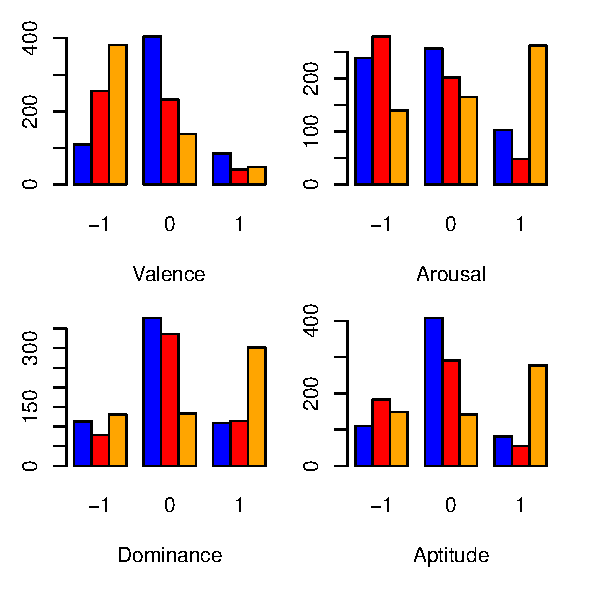
\includegraphics[width=0.9\textwidth]{retweets/figures/emotiondistribution.eps}
\caption{The distribution of each of the four parameters of emotion from the hand rated training sets for the Autism (blue), H7N9 (red) and MMR (orange) datasets.}
\label{fig:emodist}
\end{figure}


A random sample of 600 Tweets from each of the three topics was then hand rated. For rating counts, see figure \ref{fig:emodist}. Rating through a majority vote of 3 Amazon Mechanical Turk workers was considered, however agreement with a hand-coded gold standard, along with agreement between the raters, was low, with rates similar to previous work's analysis\cite{snow2008cheap}.  

These ratings were then used as a basis for training machine learning classifiers. Each of the four dimensions were evaluated independently. The attribute of a message was evaluated in two steps. First, a binary classifier determines if the text either has a relevant, emotional signal or not. That is, messages that are either irrelevant, or do not show a positive or negative polarity on the given dimension. Messages not filtered are then passed through a second binary classifier to determine if they contain a positive or negative form of the emotional dimension in question. 

To transform the text into a machine readable form, the text is converted to a binary keyword vector using scikit-learn's\cite{scikit-learn} CountVectorizer class. English stop words were removed. The tokens were converted to n-grams of size 1 to max\_n where we varied max\_n from 1 to 5. Similarly, we varied the number of times an n-gram needed to occur to be included in the final feature vector by min\_df, which we varied between 1 and 20. Additionally, we considered including or not including extra features based on the length of the tweet and the counts of numbers, exclamation marks (`!'), question marks (`?'), periods ('.'), hashtags (`\#') and at signs (`@') in the text. This results in a total of 200 possible text vectorizers considered. This keyword vector was then applied to random forest (with 5 or 10 decision trees), logistic regression, nearest neighbor, naive bayes, and support vector (with a radial basis function kernel) classifiers to classify the text as described above. 

These 1800 possible combinations were trained and evaluated against 500 hand rated messages using 5-fold cross validation. The combination that had the best accuracy, for a given step and emotional dimension, was then chosen as the ``best'' classifier. The models were then trained on the whole 500 element training/testing set and evaluated against a 100-Tweet hold out set. Additionally, we built a combined dataset that is based on the three datasets. 

We find that the models trained on the combined dataset outperform classifiers that were specialized for a specific dataset (see tables \ref{tab:emotionperformanceneutral} and \ref{tab:emotionperformancepolarity}). This is probably due to the three times increase in training data. Since the distributions tend to be non-uniform (see figure \ref{fig:emodist}), we evaluate the classifiers on the mean of the true positive and true negative rate, or 
\begin{equation}
mean\_accuracy = (\frac{TP}{TP+FN}+\frac{TN}{TN+FP})/2
\end{equation} 
where TP and TN are the number of true positives and negatives and FP and FN are the number of false positives and negatives. Note that a completely biased estimator that either always estimates positive or negative will have a mean accuracy of 0.5. Since the classifiers to find either the existence of arousal or its polarity are essentially 0.5, we are unable to develop an accurate classifier and ignore that dimension in further analysis. Additionally, we discard dominance because of the difficulty in determining polarity. Thus, we work with a two-dimensional model of emotions based on valence and aptitude. 

\begin{table}[]
\centering
\begin{tabular}{|l|l|l|p{1.15cm}|p{1.4cm}|p{1.5cm}|p{1.25cm}|}
\hline
Emotion                    & Dataset  & Best Classifier & Max n-Gram & Min Occurrences & Include Extras? & Mean Accuracy \\ \hline
\multirow{4}{*}{Aptitude}  & Autism   & Naive Bayes     & 3          & 8               & False           & 0.5385  \\ \cline{2-7} 
                           & H7N9     & Naive Bayes     & 1          & 5               & True            & 0.5280  \\ \cline{2-7} 
                           & MMR      & Naive Bayes     & 1          & 1               & False           & 0.5690  \\ \cline{2-7} 
                           & Combined & Naive Bayes     & 1          & 8               & False           & 0.6831  \\ \hline
\multirow{4}{*}{Arousal}   & Autism   & KNN             & 1          & 2               & False           & 0.4727  \\ \cline{2-7} 
                           & H7N9     & Naive Bayes     & 1          & 1               & False           & 0.5476  \\ \cline{2-7} 
                           & MMR      & KNN             & 1          & 2               & True            & 0.5073  \\ \cline{2-7} 
                           & Combined & KNN             & 1          & 15              & True            & 0.5119  \\ \hline
\multirow{4}{*}{Dominance} & Autism   & Naive Bayes     & 3          & 10              & True            & 0.7696 \\ \cline{2-7} 
                           & H7N9     & Naive Bayes     & 3          & 7               & False           & 0.4996  \\ \cline{2-7} 
                           & MMR      & Naive Bayes     & 3          & 1               & False           & 0.5471  \\ \cline{2-7} 
                           & Combined & SVM             & 3          & 10              & False           & 0.6993  \\ \hline
\multirow{4}{*}{Valence}   & Autism   & Naive Bayes     & 3          & 8               & False           & 0.6023  \\ \cline{2-7} 
                           & H7N9     & Naive Bayes     & 1          & 3               & True            & 0.5888  \\ \cline{2-7} 
                           & MMR      & KNN             & 3          & 1               & False           & 0.4940   \\ \cline{2-7} 
                           & Combined & Naive Bayes     & 3          & 14              & True            & 0.6141  \\ \hline
\end{tabular}
\caption{The performance for each of the neutral/non-neutral classifiers selected from the test/train set on the validation set.}
\label{tab:emotionperformanceneutral}
\end{table}

\begin{table}[]
\centering
\begin{tabular}{|l|l|l|p{1.15cm}|p{1.4cm}|p{1.5cm}|p{1.25cm}|}
\hline
Emotion                    & Dataset  & Best Classifier     & Max n-Gram & Min Occurrences & Include Extras? & Mean Accuracy \\ \hline
\multirow{4}{*}{Aptitude}  & Autism   & KNN                 & 1          & 1               & False           & 0.5979 \\ \cline{2-7} 
                           & H7N9     & SVM                 & 1          & 3               & False           & 0.5000           \\ \cline{2-7} 
                           & MMR      & SVM                 & 3          & 2               & False           & 0.7903   \\ \cline{2-7} 
                           & Combined & LR & 1          & 1               & True            & 0.8292  \\ \hline
\multirow{4}{*}{Arousal}   & Autism   & NB         & 1          & 5               & False           & 0.6197  \\ \cline{2-7} 
                           & H7N9     & NB         & 1          & 14              & False           & 0.5068 \\ \cline{2-7} 
                           & MMR      & KNN                 & 1          & 1               & False           & 0.6455  \\ \cline{2-7} 
                           & Combined & LR & 3          & 1               & True            & 0.7595 \\ \hline
\multirow{4}{*}{Dominance} & Autism   & NB         & 1          & 2               & True            & 0.5136 \\ \cline{2-7} 
                           & H7N9     & KNN                 & 1          & 2               & False           & 0.4298  \\ \cline{2-7} 
                           & MMR      & NB         & 3          & 1               & False           & 0.4737  \\ \cline{2-7} 
                           & Combined & KNN                 & 3          & 1               & False           & 0.5625        \\ \hline
\multirow{4}{*}{Valence}   & Autism   & LR & 1          & 1               & False           & 0.5611  \\ \cline{2-7} 
                           & H7N9     & LR & 1          & 3               & True            & 0.7384   \\ \cline{2-7} 
                           & MMR      & NB         & 1          & 16              & True            & 0.6094      \\ \cline{2-7} 
                           & Combined & LR & 3          & 1               & False           & 0.6561  \\ \hline
\end{tabular}
\caption{The performance for each of the emotion polarity classifiers selected from the test/train set on the validation set. (LR = Logistic Regression, NB = Naive Bayes)}
\label{tab:emotionperformancepolarity}
\end{table}

\section{Effects of metrics on Retweets}
\label{sec:retweetfeatures}
\subsection{Network Effects}
Of the total 947,967 tweets collected, 339,292 tweets were rated as retweets by the twitter API. An additional {39,563} hidden retweets were detected. We observe that the log-transformed lag between Tweet and Retweet is unimodal for traditional retweets, but bi-modal when we include hidden retweets. While the later peak is similar to the one detected in API retweets, the earlier peak is located at less than two seconds. It is unlikely that a human would be able to read and copy a message in this short of a time period. Instead, it would seem that this subset of hidden retweets is an attempt to make an automated account look human by copying topical conversations. Indeed, upon inspection of these accounts, we find an unusually large number of total tweets (mean = 34352.7092 Tweets per user) compared to accounts that do not show this behavior (mean = 12319.2674 Tweets per user). Future work will determine the purpose of these fake accounts. Here, we determine that these spam accounts do not actually consume or produce information -- in the traditional sense -- and we thus discard any retweets that happen within 10 seconds of the initial post (see figure \ref{fig:tweet_lag}). All analysis in the paper outside of this section is on datasets with spam accounts removed. %To test this hypothesis, we perform bi-gram analysis on the three datasets and the three types of retweets (API retweets, API + Hidden retweets, and API + Hidden retweets with spam removed) to find bi-grams that have a statistically significant relationship to \(log(\)total retweets\()\). We find that the number of bi-grams that are statistically significant at the .05 level, after bonferonni correction, are lowest when these spam accounts are not removed from the data (see figure \ref{fig:keyword_count}). This would imply that there is less predictive power for retweets with spam account included, which one would expect to see if those accounts were randomly selecting messages to repost.

As mentioned above, we model the number of times a message is propagated based on the number of users that follow the initial poster's account. The number of followers also approximates the number of people that will see a Tweet. We find that this model explains approximately 10\% of the variation in retweets (\(0.3142 \leq r  \leq 0.4169\) , p < .0001 in each case, see table \ref{tab:modelfits}). 

\begin{figure}
\centering
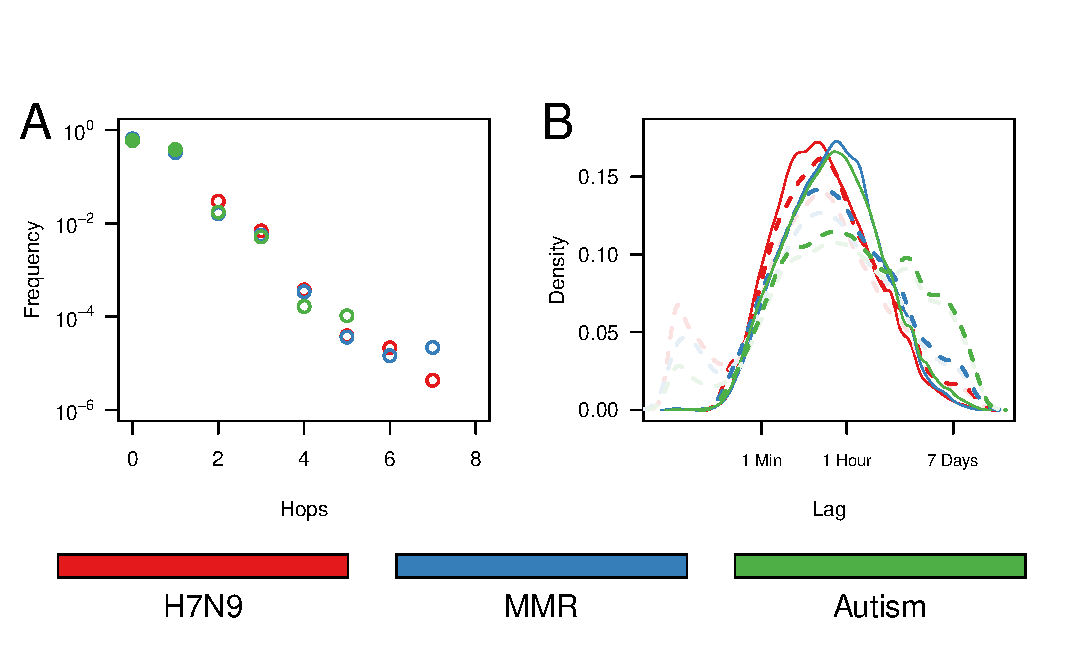
\includegraphics[width=0.9\textwidth]{retweets/figures/compareTypes.eps}
\caption{A comparison between regular retweets (solid) and hidden retweets (dashed). Hidden retweets show an exponential distribution in the distance between the tweet and it's message's origin, and regular retweets show a star topology, never being more than one hop from the origin (A). The time between when a message is posted and when a message is reposted is similar between the two types of reposts (B). However, hidden retweets may be multimodal with an additional high point in the seconds range, possibly indicating false positives.}
\label{fig:tweet_lag}
\end{figure}


\begin{table}
\centering
\begin{tabular}{l|rrr|r} \hline
Dataset & Retweets & Hidden & Retweets + Hidden & \% Hidden \ \\ \hline 
H7N9 & 74444 & 18190 & 92634 & 19.646\ \\ 
MMR & 41961 & 5627 & 47588 & 11.824\ \\ 
Autism &  215927 & 15747 & 231674 & 6.797\ \\ \hline
Total & 332332 & 39564 & 371896 & 10.639\ \\ 
\end{tabular}
\caption{The total number of retweets, hidden reproductions and total reproductions of a message.}
\label{table:retweetType}
\end{table}

\subsection{User Type Effects}
\begin{figure}
\centering
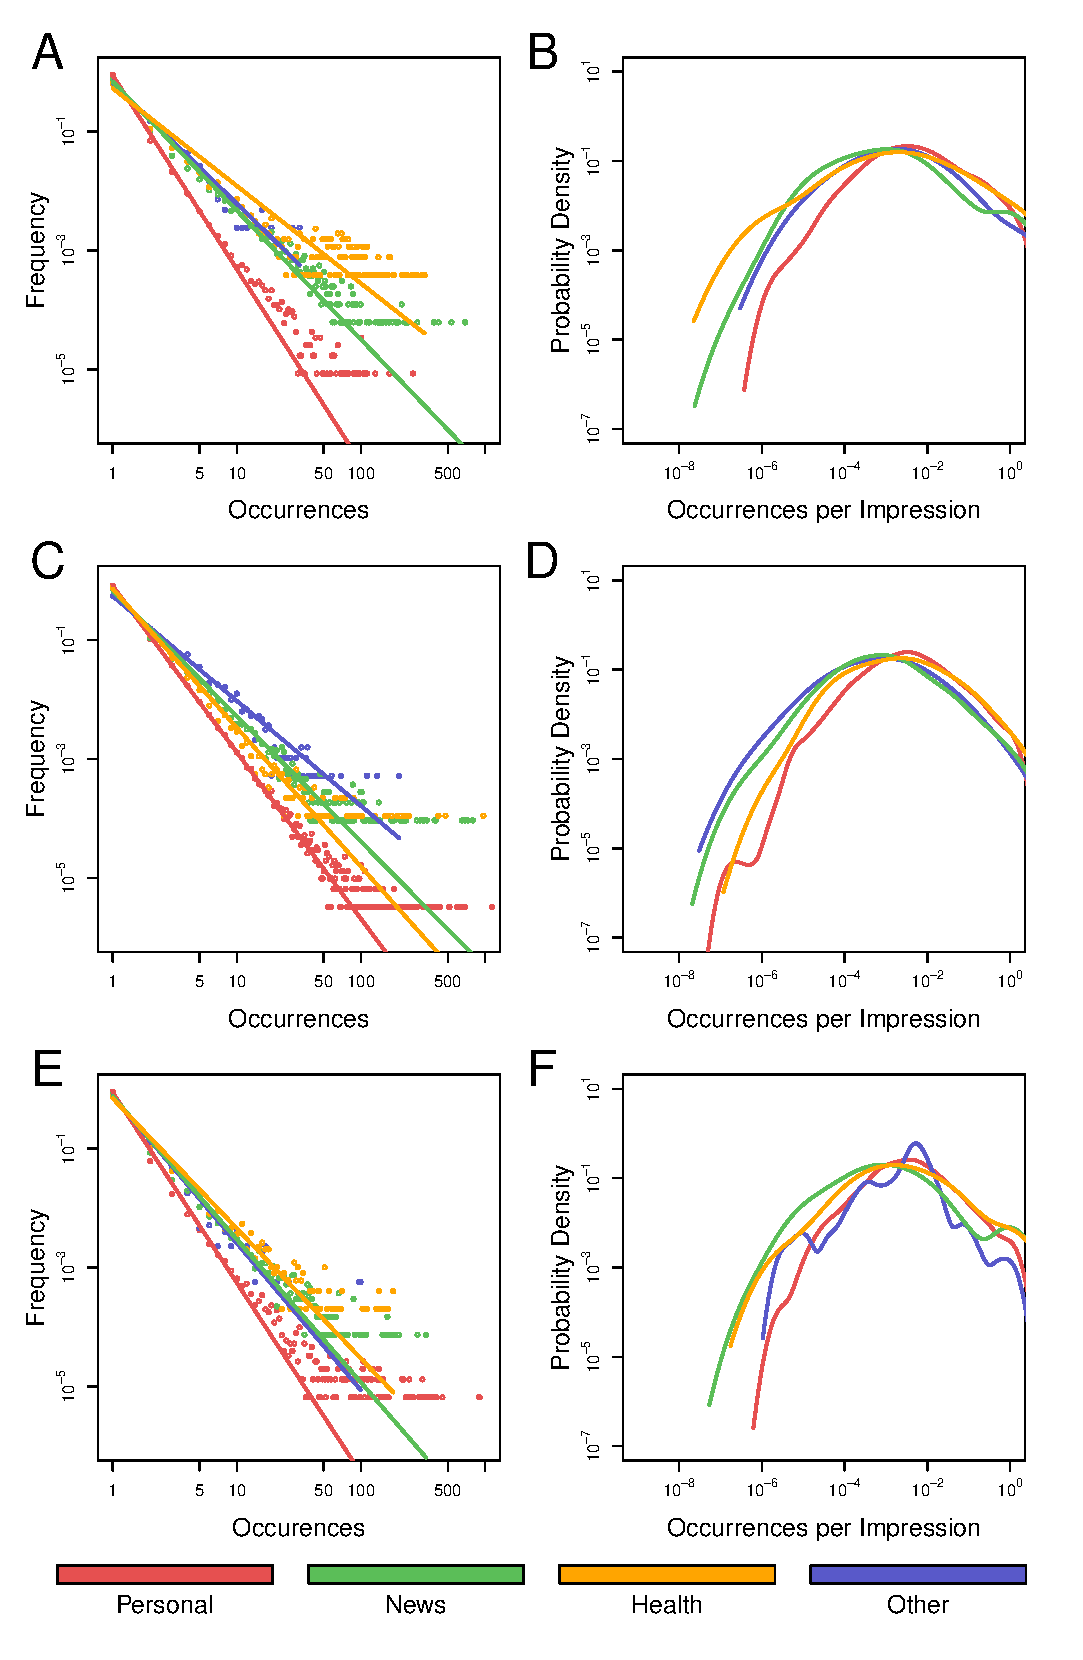
\includegraphics[width=0.5\textwidth]{retweets/figures/density_by_type.eps}
\caption{The frequency of reposts of a message by each of the four types of users (A) and the estimated probability density function of a message's posts normalize by the number of individuals that the original poster is followed by (B). Note that the non-normalized post counts have a power-law-like distribution with the dashed line representing a log-log function fit to the data. All distributions are significantly different. Occurrences are defined by the number of retweets + 1. Where we add one to account for the initial posting.}
\label{fig:type_density}
\end{figure}


\begin{figure}
\centering
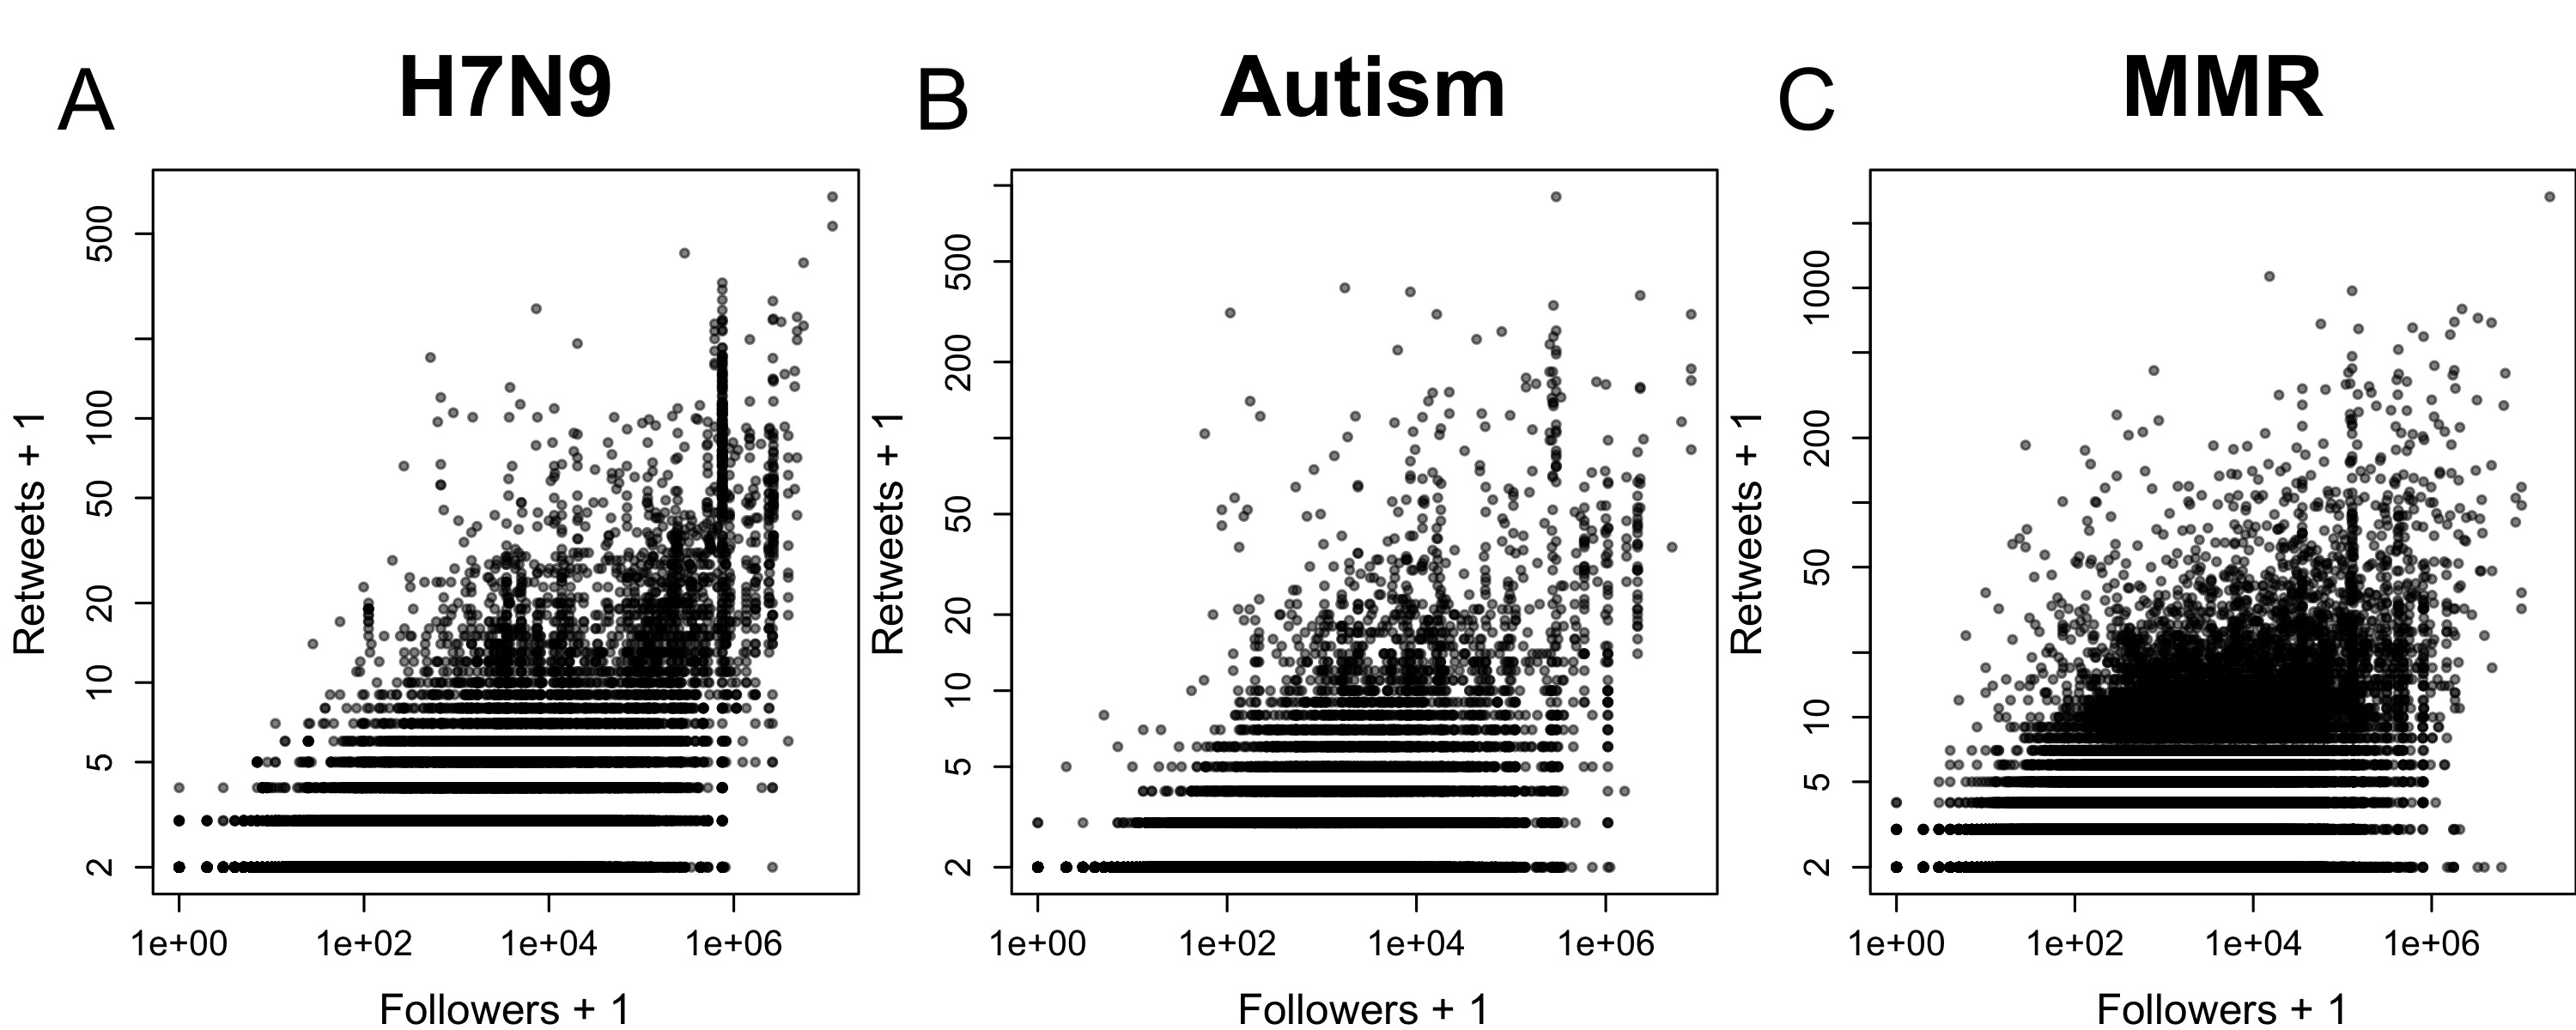
\includegraphics[width=0.9\textwidth]{retweets/figures/retweet_followers.png}
\caption{The number of times a tweet is posted based on the number of followers the original poster has.}
\label{fig:retweet_followers}
\end{figure}


\begin{table}
\centering
\begin{tabular}{c|cccc} \hline
Dataset & Personal & Other & News & Health \ \\ \hline 
H7N9 & 87602 (94.99\%) & 141 (0.15\%) & 3453 (3.74\%) & 1028 (1.11\%) \ \\ 
MMR & 57705 (95.36\%) & 195 (0.32\%) & 1651 (2.73\%) & 964 (1.59\%) \ \\ 
Autism &  269575 (96.51\%) & 940 (0.34\%) & 5264 (1.88\%) & 3535 (1.27\%) \ \\ \hline
Total &  397838 (96.38\%) & 1202 (0.29\%)  & 8851 (2.14\%) & 4896 (1.19\%) \ \\ 
\end{tabular}
\caption{The number of each type of users in each of the three datasets. Note that the total counts are lower due to duplicates between the three datasets.}
\label{table:userCounts}
\end{table}

\begin{table}
\centering
\begin{tabular}{c|rrr} \hline
User Type & Median Followers & Mean Followers & Max Followers  \ \\ \hline 
Personal & 246.0 & 1467.89   &  6424948\ \\ 
Other & 1094.5 & 15271.77 &  2503732\ \\ 
News & 2573.0 & 58323.01 & 21125687\ \\ 
Health & 302.0 & 3762.29 &   1064952\ \\ 
\end{tabular}
\caption{The number of each type of users in each of the three datasets. Note that the total counts are lower due to duplicates between the three datasets.}
\label{table:followerInfo}
\end{table}


%select sum(size-1), avg(size-1), userTypeMultiple from trees_all inner join tweets_all on trees_all.root = tweets_all.`tweetID` inner join users_all on tweets_all.`userID` = users_all.`userID` group by userTypeMultiple;
%684744	0.4485	0
%16932	1.7325	1
%212705	2.0527	2
%109540	2.5110	3

While News and Health accounts are a minority (3.33\%) of users, their messages result in 31.47\% of the retweets (see figure \ref{fig:type_density}). One may expect this as News and hHealth accounts tend to have more followers (see table \ref{table:followerInfo}). These networks effects can be controlled for by considering the frequency of retweets per follower. However, even when this control is applied, we find that Health and News accounts still tend to have more retweets. Indeed, we find that messages from health accounts tend to generate more retweets even than News accounts, despite less followers. This may be due to several factors such as end users assigning Health organizations a higher authority than News organizations or Health organizations having faster access to important news. 

As there are a fixed number of cases for the feature ACCOUNT-TYPE, we can model the effect that the type of account has on the number of retweets by using a multivariable regression based on ACCOUNT-TYPE. Since the predictive variable, ACCOUNT-TYPE is a categorical variable, this regression model can be simplified to a look up table defined as:
\begin{equation}
Retweets  =
\begin{cases}
 \text{mean(retweets of tweets from }News\text{)} & \text{If posted by }News \\
 \text{mean(retweets of tweets from }Personal\text{)} & \text{If posted by }Personal \\
 \text{mean(retweets of tweets from }Health\text{)} & \text{If posted by }Health \\
 \text{mean(retweets of tweets from }Other\text{)} & \text{If posted by }Other
\end{cases}
\end{equation}
We find that this model correlates to the true retweet count with a coorelation coefficient of between 10.73 and 25.22 for each of the datasets, corresponding to between 1.15\% and 6.36\% of the retweet variation being explained by the type of user that sent the message (See table \ref{tab:modelfits}).

\subsection{Keyword Effects}

\begin{table}[]
\centering
\begin{tabular}{|l|r|r|r|r|r|}
\hline
\multicolumn{1}{|c|}{Model}           & \multicolumn{1}{c|}{Min-N} & \multicolumn{1}{c|}{MMR} & \multicolumn{1}{c|}{H7N9} & \multicolumn{1}{c|}{Autism} & \multicolumn{1}{c|}{Combined} \\ \hline
\multirow{2}{*}{SVMR}                 & 100                        & 0.0401                   & 0.0015                    & 0.1224                      & 0.0987                        \\ \cline{2-6} 
                                      & 1000                       & 0.0232                   & -0.0157                   & 0.1066                      &     0.0642                          \\ \hline
\multirow{2}{*}{Regression Tree (2)}  & 100                        & 0.0619                   & 0.0649                    & 0.1021                      & 0.0907                        \\ \cline{2-6} 
                                      & 1000                       & 0.0914                   & 0.0590                    & 0.1036                      & 0.0969                        \\ \hline
\multirow{2}{*}{Regression Tree (5)}  & 100                        & 0.0816                   & 0.1123                    & 0.1160                      & 0.1099                        \\ \cline{2-6} 
                                      & 1000                       & 0.0998                   & 0.0958                    &                            0.1222 & 0.1025                        \\ \hline
\multirow{2}{*}{Regression Tree (10)} & 100                        & 0.0826                   & 0.0712                    & 0.1076                      & 0.0896                        \\ \cline{2-6} 
                                      & 1000                       & 0.0891                   & 0.0850                    & 0.0975                      & 0.0990                        \\ \hline
\multirow{2}{*}{Gradient Boosting}    & 100                        & \textbf{0.1800}                   & \textbf{0.1674}                    & \textbf{0.1783}                      & \textbf{0.1513}                        \\ \cline{2-6} 
                                      & 1000                       & 0.1547                   & 0.1399                    & 0.1652                      & 0.1416                        \\ \hline
\end{tabular}
\caption{Performance of various regression models to based on correlation coefficients of predicted and actual log(retweet) rates given the Tweet's textual content. Min N = Minimum number of times a word must appear to be included. SVMR = Support Vector Regression,.}
\label{tab:keywordregression}
\end{table}

Textual content appears to have a mild effect on over all retweeting rates (see table \ref{tab:keywordregression}). While this may seem surprising at first, there is a likely explanation: The words within each message are likely similar, as they are all about the same topic. For example, there are many Tweets in the autism dataset of the form ``Celebrate Autism Awareness Month.'' Since there is a wide variation in who posts these similar messages, there is also a large variation in the number of reposts each Tweet gets that is \emph{not} explained just by textual content. Later, in section \ref{sec:predictall}, we will combine the textual content with the other features to build a better preforming model. 


\subsection{Emotional Effects}

Alone, emotional content does not seem to be much of a predictor of retweet rates (see table \ref{tab:modelfits}), although the predictions are statistically significant. Here, instead, we discuss various relations between emotional content and our Twitter data. First, we find a small (\(r = -0.1185\)) but significant (\(p \leq 10^{-16}\)) relationship between valence and aptitude in our data. This may be in line with previous psychology work which assumes that these two variables are independent.\cite{plutchik2001nature}  This small relationship may be due to either biases in our classifiers or due to our large dataset providing more statistical power (a sample size of \(n\geq 274\) is required to resolve an effect of this size). Note that with an approximate \(r^2\) of 1.4\%, it is unlikely that one could infer much about one of the variables from the other, justifying the, generally employed, simplifying assumption of independence.


We find differences in the average valence and aptitude from users of different types in each of the datasets (see figure \ref{fig:user_emotion}). This shows predictable trends--such as health practitioner's appearing more knowledgeable than others--along with less expected trends. For example, we find that Health accounts tend to post more messages with negative valence while News organizations tend to stay more neutral. Additionally, note that Other accounts seem to have similar aptitude levels to that of Health accounts, but much different valence levels. We find no statistical difference (p=0.185) between aptitude in H7N9 tweets from Health and News accounts, possibly due to both groups focusing on the ``breaking'' news. Additionally, we find no statistical difference between Health, News and Personal accounts for valence about Autism (\(p\geq 0.1586\) in each case) while Other accounts have a statistically significant difference in valence from Personal ( p < 0.0001) and Health (p = 0.0006) accounts but not News accounts (p = 0.77035). All other comparisons are significant in the p < 0.001 level. All comparisons were performed using pairwise-t-tests with the Holm-Bonferroni correction for multiple tests. Additionally, we find a negative correlation between follower count and valence (Spearman's rank test \(\rho = -0.05594\), \(p < 2^{-16}\) ) and a positive relation between follower count and the aptitude of the messages (Spearman's rank test \(\rho = 0.01391\), \(p < 2^{-7}\) ).


\begin{figure}
\centering
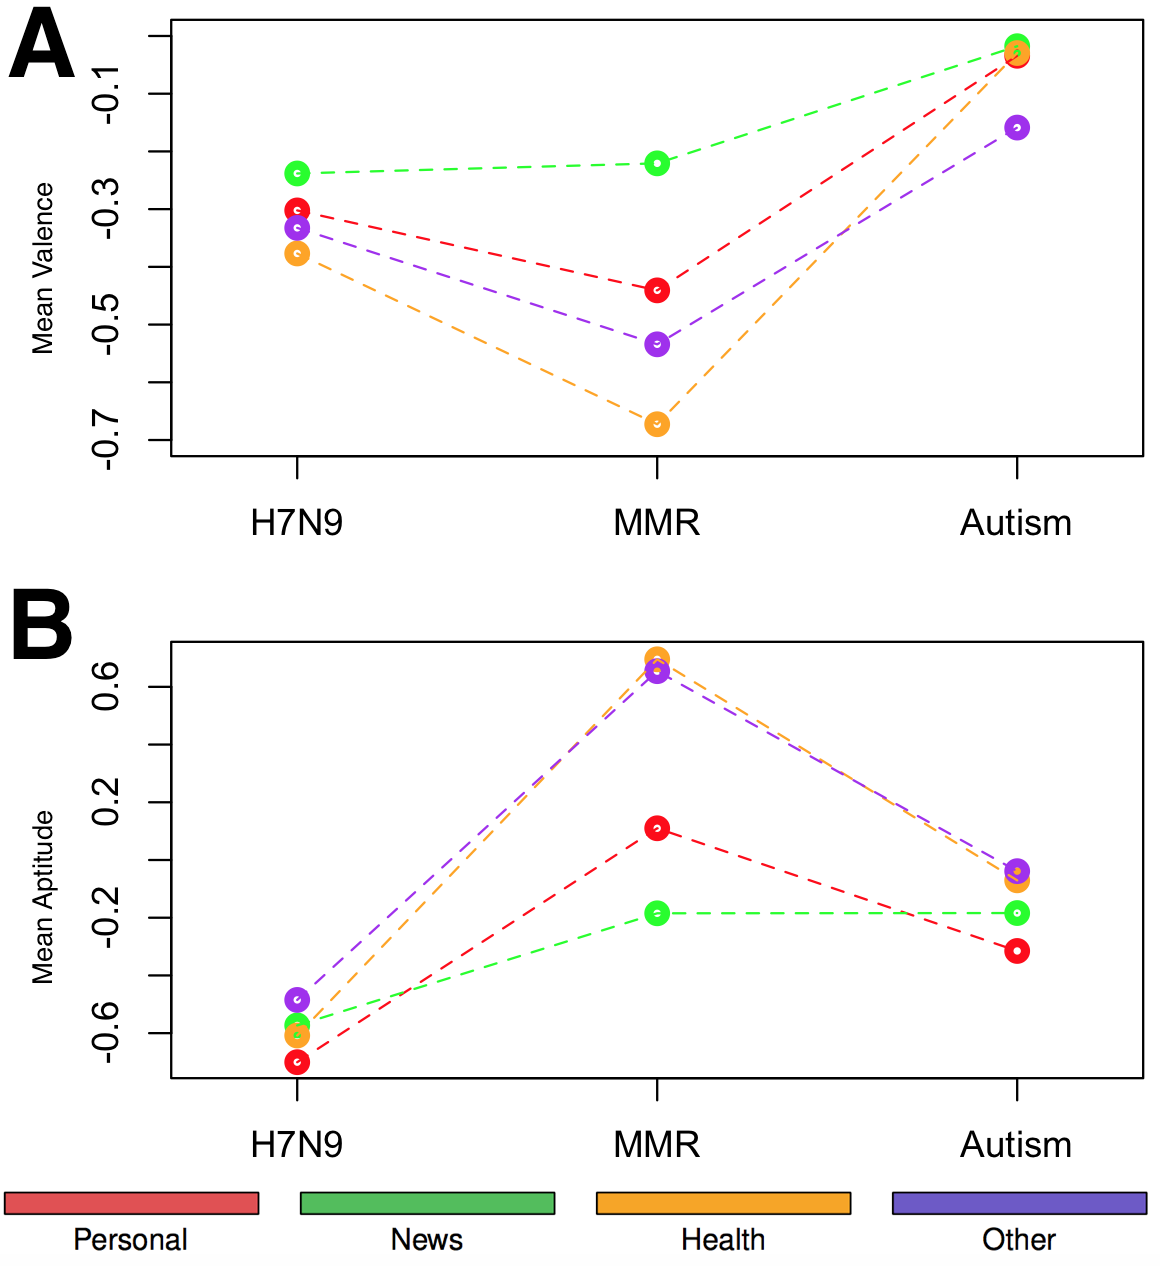
\includegraphics[width=0.95\textwidth]{retweets/figures/user_emotion_dataset.png}
\caption{The mean Valence (A) and Aptitude (B) of tweets from each of the four user types in each of our three datasets. }
\label{fig:user_emotion}
\end{figure}


\section{Prediction of Tweet Effects}
\label{sec:predictall}
We now combine the features described in section \ref{sec:retweetfeatures} to build a final predictive model. To deal with issues related to overfitting, in this chapter we worked with three subsets of each of the three datasets. We divided the datasets into an 85\%, 10\%, and 5\% train, test, and validate sub sets. All results up to this point were based on the 85\% training dataset. Since we perform model selection regarding keywords, user types, and emotions, we cannot accurately discern the models' performances. That is, since we are choosing models that have the best correlation in the training set, any final estimates of correlation would be biased. 


%\begin{table}[]
%\centering
\begin{longtable}{l|c|c|c|c|r}
\pagebreak
Data Set                   & Followers & User Type & Text & Emotion & \multicolumn{1}{l}{Correlation} \\ \hline
\multirow{15}{*}{MMR}      &           &           &      & X       & 0.0692                           \\ \cline{2-6} 
                           &           &           & X    &         & 0.1845                           \\ \cline{2-6} 
                           &           &           & X    & X       & 0.1902                           \\ \cline{2-6} 
                           &           & X         &      &         & 0.1737                           \\ \cline{2-6} 
                           &           & X         &      & X       & 0.1866                           \\ \cline{2-6} 
                           &           & X         & X    &         & 0.2559                           \\ \cline{2-6} 
                           &           & X         & X    & X       & 0.2564                           \\ \cline{2-6} 
                           & X         &           &      &         & 0.4996                           \\ \cline{2-6} 
                           & X         &           &      & X       & 0.5018                           \\ \cline{2-6} 
                           & X         &           & X    &         & 0.5095                           \\ \cline{2-6} 
                           & X         &           & X    & X       & 0.5114                           \\ \cline{2-6} 
                           & X         & X         &      &         & 0.5164                           \\ \cline{2-6} 
                           & X         & X         &      & X       & 0.5172                           \\ \cline{2-6} 
                           & X         & X         & X    &         & \textbf{0.5222}                           \\ \cline{2-6} 
                           & X         & X         & X    & X       & 0.5201                           \\ \hline
\multirow{15}{*}{H7N9}     &           &           &      & X       & 0.0169                           \\ \cline{2-6} 
                           &           &           & X    &         & 0.1712                           \\ \cline{2-6} 
                           &           &           & X    & X       & 0.1723                           \\ \cline{2-6} 
                           &           & X         &      &         & 0.2689                           \\ \cline{2-6} 
                           &           & X         &      & X       & 0.2817                           \\ \cline{2-6} 
                           &           & X         & X    &         & 0.4022                           \\ \cline{2-6} 
                           &           & X         & X    & X       & 0.4019                           \\ \cline{2-6} 
                           & X         &           &      &         & 0.6819                           \\ \cline{2-6} 
                           & X         &           &      & X       & 0.6837                           \\ \cline{2-6} 
                           & X         &           & X    &         & 0.6836                           \\ \cline{2-6} 
                           & X         &           & X    & X       & 0.6820                           \\ \cline{2-6} 
                           & X         & X         &      &         & 0.6827                           \\ \cline{2-6} 
                           & X         & X         &      & X       & 0.6846                           \\ \cline{2-6} 
                           & X         & X         & X    &         & 0.6874                           \\ \cline{2-6} 
                           & X         & X         & X    & X       & \textbf{0.6878}                           \\ \hline \pagebreak 
%Data Set                   & Followers & User Type & Text & Emotion & \multicolumn{1}{l}{Correlation} \\ \hline
\multirow{17}{*}{Autism}   &           &           &      & X       & 0.0775                           \\ \cline{2-6} 
                           &           &           & X    &         & 0.1932                           \\ \cline{2-6} 
                           &           &           &      & X       & 0.0769                           \\ \cline{2-6} 
                           &           &           & X    &         & 0.1744                           \\ \cline{2-6} 
                           &           &           & X    & X       & 0.1756                           \\ \cline{2-6} 
                           &           & X         &      &         & 0.0984                           \\ \cline{2-6} 
                           &           & X         &      & X       & 0.1243                           \\ \cline{2-6} 
                           &           & X         & X    &         & 0.2103                           \\ \cline{2-6} 
                           &           & X         & X    & X       & 0.2091                           \\ \cline{2-6} 
                           & X         &           &      &         & 0.4067                           \\ \cline{2-6} 
                           & X         &           &      & X       & 0.4144                           \\ \cline{2-6} 
                           & X         &           & X    &         & 0.4508                           \\ \cline{2-6} 
                           & X         &           & X    & X       & 0.4523                           \\ \cline{2-6} 
                           & X         & X         &      &         & 0.4097                           \\ \cline{2-6} 
                           & X         & X         &      & X       & 0.4175                           \\ \cline{2-6} 
                           & X         & X         & X    &         & 0.4533                           \\ \cline{2-6} 
                           & X         & X         & X    & X       & \textbf{0.4541}                           \\ \hline
\multirow{15}{*}{Combined} &           &           &      & X       & 0.0737                           \\ \cline{2-6} 
                           &           &           & X    &         & 0.1476                           \\ \cline{2-6} 
                           &           &           & X    & X       & 0.1474                           \\ \cline{2-6} 
                           &           & X         &      &         & 0.1412                           \\ \cline{2-6} 
                           &           & X         &      & X       & 0.1663                           \\ \cline{2-6} 
                           &           & X         & X    &         & 0.2415                           \\ \cline{2-6} 
                           &           & X         & X    & X       & 0.2406                           \\ \cline{2-6} 
                           & X         &           &      &         & 0.4844                           \\ \cline{2-6} 
                           & X         &           &      & X       & 0.4914                           \\ \cline{2-6} 
                           & X         &           & X    &         & 0.5111                           \\ \cline{2-6} 
                           & X         &           & X    & X       & 0.5109                           \\ \cline{2-6} 
                           & X         & X         &      &         & 0.4882                           \\ \cline{2-6} 
                           & X         & X         &      & X       & 0.4940                           \\ \cline{2-6} 
                           & X         & X         & X    &         & 0.5128                           \\ \cline{2-6} 
                           & X         & X         & X    & X       & \textbf{0.5130}                           \\ \hline
\caption{Combined model performance on the test sets.}
\label{tab:combinedfeatures}
\end{longtable}
%\end{table}

Since we've found that gradient boosting performs the best with the keyword studies, we base our final predictive model on gradient boosting. For each of the datasets, we build a regression model to predict log-transformed retweets based on the initial poster's log-transformed follower count, user type, textual content and emotional rating. Additionally, we consider feature selection using a factorial design to include or exclude each of these four features (see table \ref{tab:combinedfeatures}). We can also use this to estimate the predictive effects of each of the four features by comparing the decrease in model performance when a feature is removed to the full model. We find that follower count has the strongest effect with a mean decrease of 0.2866 between our datasets (see table \ref{tab:featureeffects}). 

\begin{table}[]
\centering
\begin{tabular}{l|r}
\multicolumn{1}{c|}{Included Variable} & \multicolumn{1}{c}{\(\Delta r\)} \\ \hline
Followers                              & 0.2866                       \\
User Type                              & 0.01985                      \\
Text                                   & 0.01525                      \\
Emotion                                & -0.000175                   
\end{tabular}
\caption{Decrease in mean correlation when a feature is removed from the full model.}
\label{tab:featureeffects}
\end{table}

Finally, we can select the model that predicts retweeting rates the best for each of the four models. As before, we must now score these regression models against an independent dataset. Thus we evaluate the final models against the remaining 5\% validation set and find a mean correlation of 0.5521 (see table \ref{tab:retweetfinal}), compared to a baseline of 0.3547.

\begin{table}
\centering
\begin{tabular}{l|r|r|r|r}
Model & H7N9 & Autism & MMR & Combined\\ \hline
Followers & 0.4169 & 0.3142 &0.3411 &  0.3466\\
User Type & 0.2522 & 0.1410 & 0.1073 & 0.1363 \\
Keyword & 0.1674 &  0.1738& 0.1800
 & 0.1513 \\
Emotion & 0.0221 & 0.0753 & 0.0810 & 0.0761 \\ 
\end{tabular}
\caption{The correlation coefficient for each of the models described. Models are compared with either each dataset individually or the combined dataset}
\label{tab:modelfits}
\end{table}

\begin{table}
\centering
\begin{tabular}{l|r|r|r|r}
Model & H7N9 & Autism & MMR & Combined\\ \hline
Followers & 0.1875 & 0.2128 & 0.1656 & 0.1993 \\
User Type & 0.1718 & 0.1607 &  0.2222 & 0.2027 \\
Keyword & 0.5134  & 0.5768 & 0.4862 & 0.5503\\
Emotion & 0.2497& 0.3254&0.2240 & 0.2922\\
\end{tabular}
\caption{The mean absolute error for each of the models described. Models are compared with either each dataset individually or the combined dataset}
\label{tab:modelerror}
\end{table}


\begin{table}[]
\centering
\begin{tabular}{l|r}
\multicolumn{1}{c|}{Data Set} & \multicolumn{1}{c}{\(r\)} \\ \hline
MMR                           & 0.5565                 \\
H7N9                          & 0.6665                 \\
Autism                        & 0.4667                 \\
Combined                      & 0.5185                
\end{tabular}
\caption{Performance of the final regression models on the validation datasets.}
\label{tab:retweetfinal}
\end{table}

\section{Conclusions}

In this chapter we considered the problem of retweet prediction applied to health related messages. In addition to normal retweeting behavior, we also described an additional form of message propagation based on text similarity. We then used standard features (follower count and keyword information) and novel features (account type and emotional information) to build a model that is able to predict retweet rates with up to a correlation of 0.6665 to the true retweet rates. This predictive model, along with information discussed about user type and emotional effects, could be employed by a public health practitioner to increase the reach of public health messages at minimal additional costs. 

%
%\bibliographystyle{abbrv} %%REPLACE BEFORE SUBMIT!
%\bibliography{library_nov_13_2013.bib,library2015.bib}
%
%\end{document}
